\documentclass[tikz,border=6pt]{standalone}
\usepackage{amsmath,amssymb}
\usetikzlibrary{arrows.meta,calc,decorations.markings}

\begin{document}
	
	% ============================================================
	% Concrete example:
	%   M = S^1 \subset R^2,  p = (1,0),
	%   v = (0,1) \in T_p S^1,
	%   gamma(t) = (cos t, sin t), so gamma(0)=p and gamma'(0)=v.
	% Visualization: circle (the manifold), tangent space line at p,
	% and a curve segment gamma with velocity vector v at p.
	% ============================================================
	
	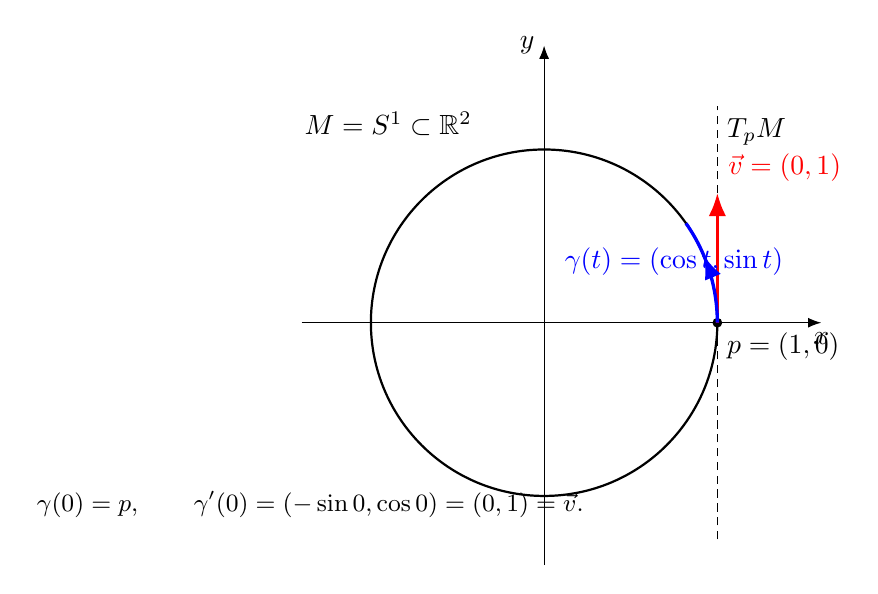
\begin{tikzpicture}[scale=2.2,>=Latex]
		
		% Axes
		\draw[->] (-1.4,0) -- (1.6,0) node[below] {$x$};
		\draw[->] (0,-1.4) -- (0,1.6) node[left] {$y$};
		
		% The manifold M = S^1
		\draw[thick] (0,0) circle (1);
		\node at (-0.9,1.15) {$M=S^{1}\subset\mathbb R^{2}$};
		
		% Point p = (1,0)
		\coordinate (p) at (1,0);
		\fill (p) circle (0.8pt);
		\node[below right] at (p) {$p=(1,0)$};
		
		% Tangent line at p: T_p S^1 is the vertical line x=1
		\draw[densely dashed] (1,-1.25) -- (1,1.25);
		\node[right] at (1,1.10) {$T_pM$};
		
		% Tangent vector v = (0,1) at p
		\draw[very thick,red,->] (p) -- ++(0,0.75) node[above right] {$\vec v=(0,1)$};
		
		% A small segment of the curve gamma(t) = (cos t, sin t)
		% Use a blue arc near t=0 (i.e., near p).
		\draw[very thick,blue,
		postaction={decorate},
		decoration={markings, mark=at position 0.65 with {\arrow{Latex}}}
		] (1,0) arc[start angle=0,end angle=35,radius=1];
		
		\node[blue] at (0.75,0.35) {$\gamma(t)=(\cos t,\sin t)$};
		
		% Show velocity interpretation at t=0
		\node[align=left] at (-1.35,-1.05) {\small
			$\gamma(0)=p,\qquad \gamma'(0)=(-\sin 0,\cos 0)=(0,1)=\vec v.$};
		
	\end{tikzpicture}
	
\end{document}
